\documentclass{standalone}
\usepackage{amssymb} % мат. символы
    \DeclareMathSymbol{\sm}{\mathbin}{AMSa}{"39} % короткий минус
    \newcommand{\mo}{\sm\!1}
\usepackage{tikz}
    \usetikzlibrary{arrows.meta}
    \usetikzlibrary{calc}
\tikzset{gdst/.style=
    {circle, draw=black!50, very thick, minimum height=1.2cm, inner sep=2pt, text centered, }, }

\begin{document}
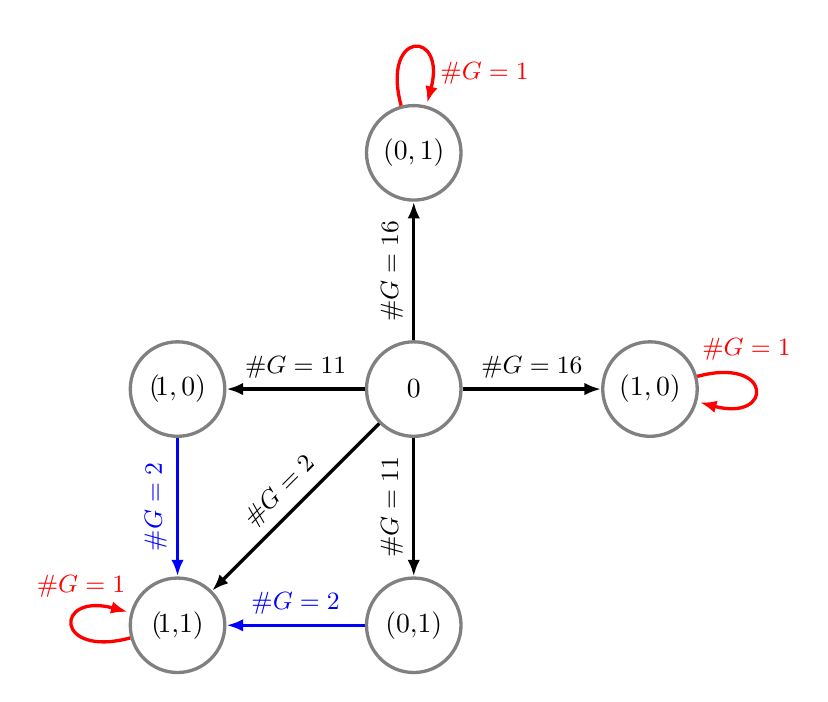
\begin{tikzpicture}
    \node[gdst, shift={(0,0)}] (f1) {${(\mo,\mo)}$};
    \node[gdst, shift={(3,0)}] (f2) {${(0,\mo)}$};
    \node[gdst, shift={(0,3)}] (f4) {${(\mo,0)}$};
    \node[gdst, shift={(3,3)}] (f5) {${0}$};
    \node[gdst, shift={(6,3)}] (f6) {${(1,0)}$};
    \node[gdst, shift={(3,6)}] (f8) {${(0,1)}$};
    \path[->,>={Latex[length=6pt]}, very thick] 
        (f1)edge[loop left, red] 
                node[shift={(0.8,0.5)}] {\small$\#G=1$} (f1)
        (f2)edge[blue]
                node[above] {\small$\#G=2$} (f1)
        (f4)edge[blue]
                node[above, rotate=90] {\small$\#G=2$} (f1)
        (f5)edge node[above, rotate=45] {\small$\#G=2$} (f1)
            edge node[above, rotate=90] {\small$\#G=11$} (f2)
            edge node[above] {\small$\#G=11$} (f4)
            edge node[above] {\small$\#G=16$} (f6)
            edge node[above, rotate=90] {\small$\#G=16$} (f8)
        (f6)edge[loop right, red] 
                node[shift={(-0.8,0.5)}] {\small$\#G=1$} (f6)
        (f8)edge[loop above, red] 
                node[shift={(0.9,-0.6)}] {\small$\#G=1$} (f8)
    ;
\end{tikzpicture}
\end{document}
% FSI_7x7_SG
% ПЕРЕСЕЧЕНИЕ ПО 78 ТОЧКАМ